\section{Theorie}
\label{sec:Theorie}

\cite{sample}
\subsection{Berechnung der Suszeptibilität}
Die magnetische Flussdichte $\vec{B}$ und die magnetische Feldstärke $\vec{H}$ hängen im Vakuum über die
Induktionskonstante $\mu_0$ zusammen.
\begin{equation}
  \vec{B} = \mu_0 \vec{H}
\end{equation}

Die magnetische Flussdichte ändert sich bei Anwesenheit von Materie um die Magnetisierung $\vec{M}$.
\begin{align}
  \vec{B} = \mu_0 \vec{H} + \vec{M}
\end{align}
Dabei ist $\vec{M}$ das mittlere magnetische Moment $\bar{\vec{\mu}}$ multipliziert der Zahl $N$ der Momente pro
Volumeneinheit.
\begin{equation}
  \vec{M} = N \mu_0 \bar{\vec{\mu}}
\end{equation}

Die Magnetisierung hängt von $\vec{H}$ und es gilt:
\begin{equation}
  \vec{M} = \mu_0 \chi \vec{H}
\end{equation}
Wobei $\chi$ die Suszeptibiliät ist und von $H$ und der Temperatur.

Paramagnetismus wird nur bei Substanzen beobachtet, welche einen nicht verschwindenden Drehimpuls besitzen.
Dieser entsteht durch die Orientierung der mit dem Drehimpuls gekoppelten magnetischen
Momente relativ zu einem äußeren Feld. Die Ausrichtung der Momente werden durch thermische Bewegungen
der atomaren Bausteine gestört, wodurch der Paramagnetismus eine temperaturabhängige Größe ist.

Der Gesamtdrehimpuls eines Atoms setzt sich aus dem
Bahndrehimpuls der Elektronenhülle, dem Eigendrehimpuls (Spin) der Elektronen und
dem Kerndrehimpuls. Der Kerndrehimpuls ist bei der Beobachtung des Bahndrehimpulses zu
vernachlässigen. Sind die Atome einem nicht allzu starken Magnetfeld ausgesetzt gilt:
\begin{align*}
  &\vec{J} = \vec{L} + \vec{S} \\
  \text{mit} \;\; &\vec{L} = \sum \vec{l_i}, \\
  &\vec{S} = \sum \vec{s_i}
\end{align*}

Dabei sind $\vec{L}$ und $\vec{S}$ die Vektorsummen die Einzeldrehimpulse sämtlicher
Elektronen in der Hülle.
Aus der Quantenmechanik folgt für die zugehörigen magnetischen Momente.
\begin{align}
  &\vec{\mu_L} = - \frac{\mu_B}{\hbar} \vec{L} \\
  &\vec{\mu_S} = -g_S \frac{\mu_B}{\hbar} \vec{S}
\end{align}

Mit $\mu_B = \frac{1}{2} \frac{e_0}{m_0} \hbar$ und $g_S$ als gyromagnetisches Verhältnis
des freien Elektrons.

Für die Beträge $|\vec{L}|$ , $|\vec{S}|$ , $|\vec{J}|$, $|\vec{\mu_L}|$ und $|\vec{\mu_S}|$ folgt aus der Quantenmechanik:
\begin{align}
  &|\vec{L}| = \sqrt{L(L+1)} \hbar \\
  &|\vec{S}| = \sqrt{S(S+1)} \hbar \\
  &|\vec{J}| = \sqrt{J(J+1)} \hbar \\
  &|\vec{\mu_L}| = \mu_B \sqrt{L(L+1)}  \\
  &|\vec{\mu_S}| = g_S \mu_B \sqrt{S(S+1)}
\end{align}

Aus Abbildung 2 lässt sich $|\vec{\mu_J}|$ berechnen.

\begin{figure}[H]
  \centering
  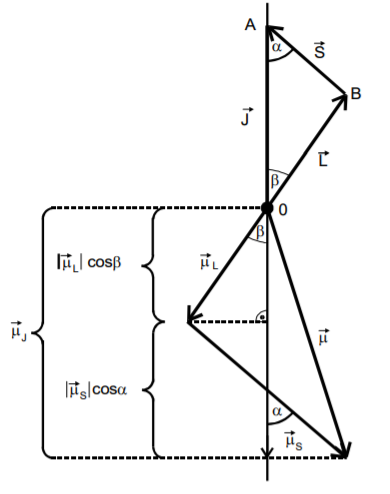
\includegraphics[height=8cm]{geometrie.PNG}
  \caption{Vektordiagramm aus den Drehimpulsvektoren und magnetischen Momenten. \cite{sample}}
  \label{fig:Linienspektrum}
\end{figure}

\begin{equation}
  |\vec{\mu_J}| = |\vec{S}| \cos{\alpha} + |\vec{\mu_L}| \cos{\beta}
\end{equation}

Wird zusätzlich $G_S$ als $2$ genähert ergibt sich:
\begin{equation}
  |\vec{\mu_J}| \approx \mu_B \sqrt{J(J+1)} \frac{3J(J+1)+ (S(S+1)-L(L+1))}{2J(J+1)}
\end{equation}

Dabei wird $g_J = \sqrt{J(J+1)} \frac{3J(J+1)+ (S(S+1)-L(L+1))}{2J(J+1)}$ als Land$\acute{\text{e}}$-Faktor bezeichnet.
Daraus folgt:
\begin{equation}
  |\vec{\mu_J}| = \mu_B g_J \sqrt{J(J+1)}
\end{equation}

Aus der Quantenmechanik folgt außerdem das Phänomen der Richtungquantelung. Dieses besagt, dass nur die Winkel
zwischen der Lage von $|\mu_J|$ und der Richtung des äußeren Magnetfeldes möglich sind, dessen Komponente
$\mu_{J_z}$ von $\mu_J$ in Feldrichtung ein ganzzahliges Vielfaches von $µ_B g_J$ ist. Somit gilt:
\begin{equation}
  \mu_{J_z} = - µ_B g_J m
\end{equation}

Dabei ist $m$ ganzzahlig und wird Orientierungszahl genannt. Es gibt $2J + 1$ Einstellmöglichkeiten
des atomaren magnetischen Momentes relativ zu einer äußeren Feldrichtung und zu jeder dieser Einstellrichtungen
gehört eine bestimmte potentielle Energie $E_m$:
\begin{equation}
  E_m = - \vec{\mu_J} \vec{B} = \mu_{J_z} B = \mu_B g_J m B
\end{equation}

Die Magnetisierung lässt sich dann aus der Häufigkeit berechnen, mit der eine bestimmte Orientierung
der magnetischen Momente auftritt. Diese wird mit  dem
zugehörigen Betrag des Momentes multipliziert und dann über alle vorkommenden
Orientierungen summiert. Daraus ergibt sich:
\begin{align}
  &M = \frac{1}{3} \mu_0 \mu_B^2 g_J^2 N \frac{J(J+1)B}{kT} \\
  &\chi = \frac{\mu_0 \mu_B^2 g_J^2 N J(J+1)}{3kT}
\end{align}

Dabei ist $k$ die Boltzmann-Konstante und $T$ die Temperatur. Gleichung (18) zeigt eine
Proportionaliät zwischen $\chi$ und $\frac{1}{T}$, welche als Curiesches Gesetz des Paramgnetismus bezeichnet wird.

Selten-Erd-Elemente zeigen besonders starken Paramagnetismus. Dafür sind die 4f-Elektronen in der Atomhülle
verantwortlich. Deren Anordnung in der unabgeschlossenen 4f-Schale und der daraus resultierende Gesamtdrehtimpuls
lässt sich durch die Hundschen Regeln beschrieben:
1. Die Spins $\vec{s_i}$ der Elektronen addieren sich zum maximalen Gesamtspin $\vec{S} = \sum \vec{s_i}$ der nach dem Pauli-Prinzip möglich ist.

2. Die Bahndrehimpulse $\vec{l_i}$ der Elektronen addieren sich zum maximalen Gesamtbahndrehimpuls $\vec{L} = \sum \vec{l_i}$ der mit
dem Pauli-Prinzip und der ersten Regel verträglich ist.

3. Der Gesamtdrehimpuls $\vec{J}$ ist für weniger als halb gefüllte Schalen $\vec{J} = \vec{L}- \vec{S}$ und für mehr als halb gefüllte Schalen
$\vec{J} = \vec{L} + \vec{S}$ .


\subsection{Apparatur zur Messung der Suszeptibilität}
Die Suszeptibilität einer Probe wird durch die Induktivitätsmessung zweier Spulen vorgenommen.

\begin{figure}[H]
  \centering
  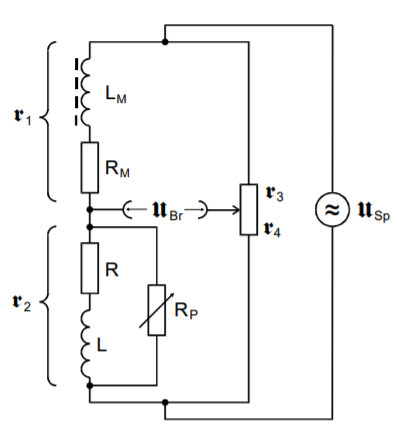
\includegraphics[height=8cm]{brueckenschaltung.PNG}
  \caption{Schaltung zur Bestimmung der Suszeptibilität einer Probe. \cite{sample}}
  \label{fig:bruecke}
\end{figure}

Dabei wird aus der gemessenen Brückenspannung $U_{Br}$ die Suszeptibilität bestimmt. Für hinreichend große Messfrequenzen
$(\omega^2 L^2) \gg R^2)$ gilt nach dem Abgleichen der Spulen und das befüllen einer Spule mit der Probe:
\begin{align}
  \chi(\omega \rightarrow \infty) = 4 \frac{F}{Q} \frac{U_{Br}}{U_{Sp}}
\end{align}
Dabei ist $F$ der Spulenquerschnitt, $Q$ der Querschnitt der Probe, welche in die Spule gefüllt wird und $U_{Sp}$ die
Speisepannung.

Eine zweite Methode ist, nachdem Befüllen einer Spule mit der Probe erneut abzugleichen, sodass $U_{Br} = 0$ ist. Aus
der Änderung der Abgleichelemente wird die Suszeptibilität berechnet. Für die Suszeptibilität gilt dann:
\begin{align}
  \chi = 2 \frac{\Delta R}{R_3} \frac{F}{Q}
\end{align}
Wobei $R_3$ der Widerstand am Potentiometer ist und $\Delta R$ die Änderung des Widerstandes ist, um die
Brückenspannung nachdem dem einfüllen der Probe wieder auf Null zu senken.

Für $Q$ muss in diesem Fall $Q_{real} = \frac{M_p}{L \rho_w}$. Dabei ist $M_p$ die Masse der Probe und $\rho_w$ die Dichte
eines Einkristalles der Probe.


An den Ausgangsklemmen der Brückenspannung ist eine Störspannung zu messen, welche die Brückenspannung überdeckt. Die
zu messene Spannung ist jedoch eine monofrequente Signalspannung. Mit einem Filter, welcher die Signalspannung herausfiltert
wird das Problem gelöst.
